% Exercise 7: Figures/Pictures in your report

% 1. Lets start by creating a report document! use \documentclass{report} 
\documentclass{report} 
% 2. Uncomment the following preamble packages to load options for figures
% Preamble
%\usepackage{graphicx} % for figures
%\usepackage{subfig} % for subplots
%\usepackage{wrapfig} %Wrap around figures
%\usepackage{lscape} %for landscape
%\usepackage{hyperref} % Hyperreferencing 
%\usepackage{url} % URL
%\usepackage{sidecap} %Side captions

% 3. Create a title and author using \title and \author{names}. Begin document, and insert the title using \maketitle
\title{King's College, Cambridge}
\author{Krishna Kumar \thanks{grad.computing@kings.cam.ac.uk}}

% 4. Uncomment to insert list of figures: \listoffigures

\begin{document}
\maketitle
\listoffigures
\clearpage

\section{King's College, Cambridge}


% 5. To create a href and url use \href{name@mail.com}{mail} and use \url{www.website.com}

My email ID is: %\href{name@mail.com}{mail}\\

My personal website is at: %\url{http://www.kings.cam.ac.uk}\\

King's College is a constituent college of the University of Cambridge, England. The college's full name is ``The King's College of our Lady and Saint Nicholas in Cambridge", but it is usually referred to simply as ``King's" within the University.

The college was founded in 1441 by King Henry VI, soon after its sister college in Eton. However, the King's plans for the college were disrupted by the civil war and resultant scarcity of funds, and his eventual deposition. Little progress was made on the project until in 1508 King Henry VII began to take an interest in the college, most likely as a political move to legitimise his new position. The building of the college's chapel, begun in 1446, was finally finished in 1544 during the reign of King Henry VIII.


% 6. To create a figure use the float \begin{figure} \end{figure}. Inserting a picture requires graphicx package. 
% 7. To include the figure use \includegraphics[options]{name}. name usually specifies the location of the figure. Recommend using a directory to hold all the figures. Options include the size / width. 
% 8. Uncomment [htbp!] the options specify location of the figure. [h-here, t-top, b-bottom, p-para and !-override] try using one at a time and see the location of figures. 
% LaTeX usually tries to place the figures closer to where it has been referenced!

\begin{figure} %[htbp!] 
\centering    %remove comment
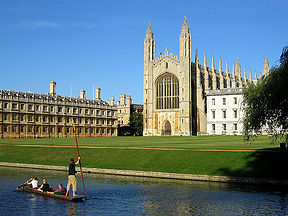
\includegraphics[scale=1.0]{Pictures/Kings.jpg}
\caption[King's College Cambridge]{``The King's College of our Lady and Saint Nicholas in Cambridge", but it is usually referred to simply as ``King's" within the University of Cambridge, England.}
\label{fig:Kings}
\end{figure}

% 9. Referencing the figure is done using \ref{unique_label}. Label of the figures should be unique. 

King's College Chapel (see ~Fig.\ref{fig:Kings}) is regarded as one of the greatest examples of late Gothic English architecture. It has the world's largest fan-vault, and the chapel's stained-glass windows and wooden chancel screen are considered some of the finest from their era. The building is seen as emblematic of Cambridge. The chapel's choir, composed of male students at King's and choristers from the nearby King's College School, is one of the most accomplished and renowned in the world. Every year on Christmas Eve the Festival of Nine Lessons and Carols (a service created by a Dean of King's especially for the college) is broadcast from the chapel to millions of listeners worldwide.

King's was founded in 1441 by King Henry VI. His first design was modest, but by 1445 was intended to be a magnificent display of royal patronage. There were to be a Provost and seventy scholars, occupying a substantial site in central Cambridge whose drastic clearance involved the closure of several streets. The college was granted a remarkable series of feudal privileges, and all of this was supported by a substantial series of endowments from the King.

King Henry VI had admired the achievements of William of Wykeham, who had founded the twin colleges of New College, Oxford (King's College's Sister College) and Winchester College in 1379. He subsequently modelled the establishment of King's and Eton College upon the successful formation of Wykeham's institutions. Indeed, the link that King's College and Eton College share is a direct copy of the link shared between New College and Winchester College. The four colleges continue to share formal ties to this day.

Originally, the college was to be specifically for boys from Eton College. It was not until 1865 that the first non-Etonian undergraduates arrived to study at King's, and the first fellow to have not attended Eton was elected in 1873. \\

% 10. Use parbox to create two colums with text and a figure. See the use of width=0.25\texwidth. Try to vary the value and see how the alignment changes.


%\parbox{0.3\textwidth}{ 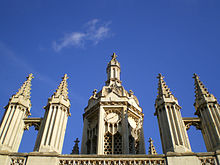
\includegraphics[width=0.25\textwidth]{Pictures/clock.jpg}}
%\parbox{0.6\textwidth}{The connection with Eton is now weak, but a scholarship to attend the college, exclusively available to students from Eton, is still awarded each year. The Gatehouse, built in the neo-Gothic style, as seen from King's Parade. The Gatehouse clock, as seen from the Great Court.}

\vspace{10pt}
The very first buildings of the college, now part of the Old Schools, were begun in 1441, but by 1443 the decision to build to a much grander plan had been taken (see Fig.~\ref{fig:pan}). That plan survives in the 1448 Founders Will describing in detail a magnificent court with a chapel on one side. But within a decade, civil war (the Wars of the Roses) meant that funds from the King began to dry up. By the time of his deposition in 1461, the chapel walls had been raised 60 ft high at the east end but only 8 ft at the west; a building line which can still be seen today as the boundary between the lighter stone below and the darker above. Work proceeded sporadically until a generation later in 1508 when the Founder's nephew King Henry VII was prevailed upon to finish the shell of the building. The interior had to wait a further generation until completion by 1544 with the aid of King Henry VIII.

% 11. Insert a figure "Pictures/Panorama.jpg" covering 85\% of text width. Add captions and insert a label called fig:pan.


It has been speculated that the choice of the college as a beneficiary by the two later Henrys was a political one, with Henry VII in particular concerned to legitimate a new, post-civil war Tudor regime by demonstrating patronage of what was by definition the King's College. Later building work is marked by an uninhibited branding with the Tudor rose and other symbols of the new establishment, quite against the precise instructions of the Founders Will. Henry VI is not completely forgotten at the College, however, the Saturday after the end of Michaelmas term each year is Founder's Day which begins with a Founder's Eucharist in the chapel, followed by a Founder's Breakfast with ale and culminating in a sumptuous dinner in his memory called ``Founder's Feast" to which all members of College in their last year of studies are invited.


% 12. Figures with sidecaption can be created using the SCfigure environment. It requires sidecap package.

%\begin{SCfigure}
%\centering
%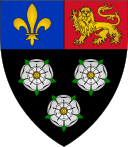
\includegraphics[scale=0.85]{Pictures/crest.png}
%\caption{King's college crest}
%\label{fig:crest}
%\end{SCfigure}

King's College Chapel is regarded as one of the greatest examples of late Gothic English architecture. It has the world's largest fan-vault, and the chapel's stained-glass windows and wooden chancel screen are considered some of the finest from their era. The building is seen as emblematic of Cambridge. The chapel's choir, composed of male students at King's and choristers from the nearby King's College School, is one of the most accomplished and renowned in the world. Every year on Christmas Eve the Festival of Nine Lessons and Carols (a service created by a Dean of King's especially for the college) is broadcast from the chapel to millions of listeners worldwide. King's was founded in 1441 by King Henry VI. His first design was modest, but by 1445 was intended to be a magnificent display of royal patronage. There were to be a Provost and seventy scholars, occupying a substantial site in central Cambridge whose drastic clearance involved the closure of several streets. 

The college was granted a remarkable series of feudal privileges, and all of this was supported by a substantial series of endowments from the King. King Henry VI had admired the achievements of William of Wykeham, who had founded the twin colleges of New College, Oxford (King's College's Sister College) and Winchester College in 1379. He subsequently modelled the establishment of King's and Eton College upon the successful formation of Wykeham's institutions. Indeed, the link that King's College and Eton College share is a direct copy of the link shared between New College and Winchester College. The four colleges continue to share formal ties to this day. Originally, the college was to be specifically for boys from Eton College. It was not until 1865 that the first non-Etonian undergraduates arrived to study at King's, and the first fellow to have not attended Eton was elected in 1873. \\

% 13. Wrap figure package allows to wrap text around a picture. Try to modify the whitespace between the text and the figure use \vspace{length}

%\begin{wrapfigure}{r}{0.5\textwidth}
%%\vspace{-10mm} % Remove white space
%  \begin{center}
%    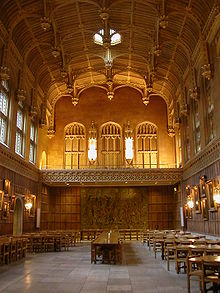
\includegraphics[width=0.48\textwidth]{Pictures/dining.jpg}
%  \end{center}
%  \caption{Hall}
%\end{wrapfigure}

The very first buildings of the college, now part of the Old Schools, were begun in 1441, but by 1443 the decision to build to a much grander plan had been taken (see Fig.~\ref{fig:pan}). That plan survives in the 1448 Founders Will describing in detail a magnificent court with a chapel on one side. But within a decade, civil war (the Wars of the Roses) meant that funds from the King began to dry up. By the time of his deposition in 1461, the chapel walls had been raised 60 ft high at the east end but only 8 ft at the west; a building line which can still be seen today as the boundary between the lighter stone below and the darker above. Work proceeded sporadically until a generation later in 1508 when the Founder's nephew King Henry VII was prevailed upon to finish the shell of the building. The interior had to wait a further generation until completion by 1544 with the aid of King Henry VIII. The college was granted a remarkable series of feudal privileges, and all of this was supported by a substantial series of endowments from the King. King Henry VI had admired the achievements of William of Wykeham, who had founded the twin colleges of New College, Oxford (King's College's Sister College) and Winchester College in 1379. He subsequently modelled the establishment of King's and Eton College upon the successful formation of Wykeham's institutions. Indeed, the link that King's College and Eton College share is a direct copy of the link shared between New College and Winchester College. The four colleges continue to share formal ties to this day. Originally, the college was to be specifically for boys from Eton College. It was not until 1865 that the first non-Etonian undergraduates arrived to study at King's, and the first fellow to have not attended Eton was elected in 1873. \\

\newpage

% 14. A figure can be flipped in LaTeX using \reflectbox{\includegraphics{name}} to flip! 
% 15. Note the location of \caption in both the figures!

%\begin{figure}[h!]
%  \caption{A picture of King's College Chapel.}
%  \centering
%    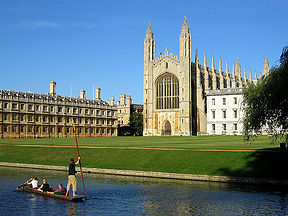
\includegraphics[width=0.5\textwidth]{Pictures/Kings.jpg}
%\end{figure}
% 
%\begin{figure}[h!]
%  \centering
%    \reflectbox{%
%      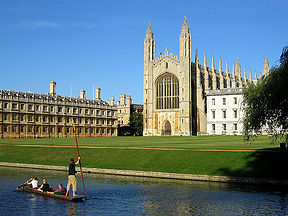
\includegraphics[width=0.5\textwidth]{Pictures/Kings.jpg}}
%  \caption{A picture of the same King's College
%  			Chapel reflection!}
%\end{figure}

\clearpage

% * Note the use of landscape environment to set the page set-up as landscape

\begin{landscape}

\section*{Subplots}
I can site Wall-E (see Fig.~\ref{fig:WallE}) and Minions in despicable me (~\ref{fig:Minnion}) or I can site the whole figure as (Fig.~\ref{fig:animations})


% 16. A subplot can be created inside the figure environment using \subfloat and \includegraphics{name} for each subfigure.

%\begin{figure}
%  \centering
%  \subfloat[A Tom and Jerry]{\label{fig:TomJerry}
\includegraphics[width=0.5\textwidth]{Pictures/TomandJerry.jpg}}                
%  \subfloat[A Wall-E]{\label{fig:WallE}
\includegraphics[width=0.5\textwidth]{Pictures/WallE.jpg}}
%  \subfloat[A Minion]{\label{fig:Minnion}
\includegraphics[width=0.5\textwidth]{Pictures/minion.jpg}}
%  \caption{Best Animations}
%  \label{fig:animations}
%\end{figure}
%\end{landscape}


\end{document}